
\subsubsection{【概要】}
dmath,math環境をequationに変換

\subsubsection{【入力:hiki】}\begin{quote}\begin{verbatim}
mathがうまくいくかどうかの検討用サンプルです.
{{dmath 'f_x'}}
さらにinlineで{{math 'x_i'}}なんかもできるといいのですが.
\end{verbatim}\end{quote}
mathがうまくいくかどうかの検討用サンプルです.
\begin{equation}
f_x
\end{equation}
さらにinlineで$x_i$なんかもできるといいのですが.

\subsubsection{【出力:latex】}\begin{quote}\begin{verbatim}
\begin{document}
mathがうまくいくかどうかの検討用サンプルです.
\begin{equation}
f_x
\end{equation}
さらにinlineで$x_i$なんかもできるといいのですが.
\end{verbatim}\end{quote}\begin{description}
\item[注2016/02/20] このあたりでhiki, rubyを指定するとlistingsがうまく処理できない.preformatted\_without\_styleで対応.

\end{description}
\begin{figure}[htbp]\begin{center}
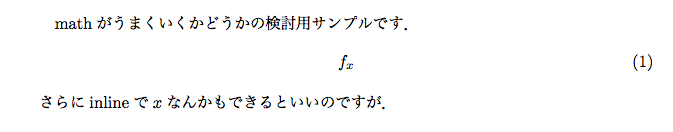
\includegraphics[width=6cm]{./Math.png}
\caption{}
\label{default}\end{center}\end{figure}
\subsubsection{【コード解説】}
\paragraph{evaluate\_plugin\_block}
すこしトリッキーだったので,メモです.
\begin{lstlisting}[style=customRuby]
  def evaluate_plugin_block(str, buf = nil)
    buf ||= @output.container
    str.split(/(\0\d+\0)/).each do |s|
      if s[0, 1] == "\0" and s[-1, 1] == "\0"
        buf << @output.inline_plugin(plugin_block(s[1..-2].to_i))
      else
        buf << @output.text(s)
      end
    end
    buf
  end
\end{lstlisting}
としてinline\_pluginはblock\_pluginと違った扱いになっています.bufに一度溜め込んでそれを@fに吐いているようです.
そこで,@output.inline\_pluginで行き着く先が,LatexOutputの
\begin{lstlisting}[style=customRuby]
  def inline_plugin(src)
    tmp=[]
    if ( /(\w+)\((.+)\)/ =~ src ) or ( /(\w+).\'(.+)\'/ =~src ) or (/(\w+)/ =~ src)
      tmp = [$1,$2]
    end

    case tmp[0]
    when 'dmath'
      "\\begin{equation}\n#{tmp[1]}\n\\end{equation}"
    when 'math'
      "\$#{tmp[1]}\$"
    else
      %Q(<span class="plugin">{{#{src}}}</span>)
    end
  end
\end{lstlisting}
としてmath,dmathを処理しています.必要ならそれ以外のinlineもここに付け足すことで対応できます.

\paragraph{snake\_nameがlatexで引っかかる}
math環境の移し替えはうまくいったが,underscore\_namesがすべて引っかかるequationとして引っかかる.
\begin{quote}\begin{verbatim}
\usepackage{underscore}
\end{verbatim}\end{quote}
だけでもできるようだが,できればto\_latexで対応したい.ということで,paragraphにescape\_snake\_namesを入れた.

paragraphはpreformattedからは呼ばれない.しかし,\verb|$$|や\verb|\begin{equation}...\end{equation}|が含まれる.そこで
一旦全置換してそこだけ戻すようにした.gsubのなかでなんどもできるか自信がなくて.二重のgsubにしているが...
\begin{lstlisting}[style=customRuby]
  def escape_snake_names(str)
    str.gsub!(/_/,"\\_")
    str.gsub!(/\$.+?\$/){ |text| text.gsub!(/\\_/,"_")  }
    str.gsub!(/equation.+?equation/m){ |text| text.gsub!(/\\_/,"_") }
  end

  def paragraph(lines)
    lines.each{|line| line = escape_snake_names(line) }
    @f << "#{lines.join("\n")}\n\n"
  end
\end{lstlisting}
gsub!で置換できなかったときには,nilが返るので対応.なんかえらく冗長.
\begin{lstlisting}[style=customRuby]
  def escape_snake_names(str)
    str.gsub!(/_/,"\\_")
    str.gsub!(/\$.+?\$/){ |text|
      if text =~ /\\_/ then
        text.gsub!(/\\_/,"_")
        else
        text
      end
    }
    str.gsub!(/equation.+?equation/m){ |text|
      if text =~ /\\_/ then
        text.gsub!(/\\_/,"_")
        else
        text
      end
    }
    str
  end
\end{lstlisting}
\paragraph{escape\_snake\_namesを改良(2016/02/14)}
gemへの公開にあたって冗長部を簡略化.verbだけはここを切り出した検証とは違う.testにuriを埋め込んでverb変換とsnakeを検証.
\begin{lstlisting}[style=customRuby]
  def escape_snake_names(str)
    str.gsub!(/_/,"\\_")
    patterns = [/\$(.+?)\$/ , /\\verb\|(.+?)\|/, /equation(.+?)equation/m ]
    patterns.each{|pattern|
      str.gsub!(/\\_/,"_")    if str.match(pattern)
    }
    str
  end
\end{lstlisting}
\paragraph{escape\_snake\_namesを再改良(2016/02/16)}
underscoreではincludeなどでsnake\_named\_fileも変換してしまい,だめ.hiki2latexで対応.

上のやり方では,うまくいかない場合が存在.元へ戻す.
\begin{lstlisting}[style=customRuby]
def escape_snake_names(str)
    str.gsub!(/_/,"\\_")
    patterns = [/\$(.+?)\$/ , /\\verb\|(.+?)\|/, /equation(.+?)equation/m ]
    patterns.each{|pattern|
#      str.gsub!(/\\_/,"_")    if str.match(pattern)                                                                                   
      str.gsub!(pattern){|text|
        if text =~ /\\_/ then
          text.gsub!(/\\_/,'_')
        else
          text
        end
      }
    }
    str
  end
\end{lstlisting}
さらに
tableでescape\_snake\_namesを通ってなかった.
\begin{quote}\begin{verbatim}
#        buf << "#{ele} &"
       buf << escape_snake_names(ele)+" &"
\end{verbatim}\end{quote}
\subsubsection{【copyright】}
cc by Shigeto R. Nishitani, 2015

